\documentclass{article}

% --- packages ---
\usepackage[utf8]{inputenc}
\usepackage[T1]{fontenc}
\usepackage{amsmath,amssymb,amsfonts,amsthm}
\usepackage{graphicx}
\usepackage{booktabs}
\usepackage{hyperref}
\usepackage{float}
\usepackage{xcolor}
\usepackage[margin=1in]{geometry}
\usepackage{natbib}
\usepackage{subcaption}
\usepackage{tikz}
\usepackage{pgfplots}
\pgfplotsset{compat=1.17}
\usetikzlibrary{positioning,arrows.meta,calc,fit,backgrounds,shapes.geometric}

% --- theorem environments ---
\newtheorem{definition}{Definition}
\newtheorem{proposition}{Proposition}
\newtheorem{remark}{Remark}

% --- macros ---
\newcommand{\R}{\mathbb{R}}
\newcommand{\E}{\mathbb{E}}
\newcommand{\rms}{\textsc{RMSNorm}}
\newcommand{\bandrms}{\textsc{BandRMS}}
\newcommand{\zcrms}{\textsc{ZeroCenteredRMSNorm}}
\newcommand{\zcband}{\textsc{ZeroCenteredBandRMSNorm}}
\newcommand{\layernorm}{\textsc{LayerNorm}}
\newcommand{\batchnorm}{\textsc{BatchNorm}}

% --- colors for charts ---
\definecolor{baselinegray}{RGB}{127,127,127}
\definecolor{bandorange}{RGB}{255,127,14}
\definecolor{zcblue}{RGB}{31,119,180}
\definecolor{combopurple}{RGB}{148,103,189}
\definecolor{passgreen}{RGB}{44,160,44}
\definecolor{failred}{RGB}{214,39,40}

\title{Is the Band Worth It? A Multi-Seed Comparison of RMSNorm Variants\\
\large{An empirical evaluation of \bandrms{}, \zcrms{}, and \zcband{} across five regimes}}

\author{
  Nikolas Markou \\
  \texttt{nikolasmarkou@gmail.com}
}

\date{}

\begin{document}

\maketitle

% ============================================================================
\begin{abstract}
We empirically evaluate three increasingly elaborate variants of \rms{} normalization --- \bandrms{} (output magnitude constrained to a learnable band $[1-\alpha,\,1]$), \zcrms{} (mean subtracted before RMS rescaling), and \zcband{} (both modifications combined) --- against vanilla \rms{} across five settings: ViT-pico on CIFAR-10, ResNet-18 on CIFAR-100, a 4-layer pre-norm transformer on IMDb, a 24-block deep residual stack under mixed precision, and a layer-level synthetic microbenchmark.
We run $n{=}5$ random seeds per cell and report mean~$\pm$ std, 95\% bootstrap CI, and a paired sign-flip permutation $p$-value (B${=}10{,}000$, Phipson-Smyth corrected) against the \rms{} baseline.
Four mechanistic probe callbacks log per-epoch activation mean, per-sample RMS distribution, weight $L_2$ trajectory, and gradient norm at every normalization layer, directly testing each variant's specific theoretical claim.
Three findings emerge.
First, \textbf{the band constraint by itself produces no measurable benefit on any task we tested}: \bandrms{} mechanistically confines output RMS to $[0.9, 1.0]$ as advertised, but yields zero accuracy or loss improvement over \rms{} across all five experiments and ten parameter-matched cells.
Second, \textbf{zero-centering is the operative innovation}: \zcrms{} produces near-zero output mean ($|\E[x]|$ reduced 30--500$\times$) and translates this into a decisive $+41.8$\,pp swing on ResNet/CIFAR-100 (random $\to$ learning), a $-28\%$ validation-loss reduction with $2.8\times$ lower seed variance on the deep-fp16 stack, and modest lifts elsewhere.
Third, \textbf{combining both gives the tightest variance} ($62\%$ lower std on ViT/CIFAR-10) and the best accuracy on the two vision tasks, but the band's tightness slightly hurts on the 24-block deep stack.
We further document a cross-experiment dissociation: shallow pre-norm transformers are mechanistically insensitive to norm-variant choice (E3 universal null within $\pm 0.1$\,pp), while post-norm-like or deep regimes are where residual-stream DC drift dominates and zero-centering becomes critical.
A 1-line fp16 cast bug in the original \bandrms{} and \zcband{} implementations is reported and fixed; without it, mixed-precision input crashes the multiply against the fp32 normalized tensor.
\end{abstract}

% ============================================================================
\section{Introduction}
\label{sec:intro}

The default normalization layer in modern transformers is \layernorm{}~\citep{ba2016layer}: $x \mapsto \gamma \odot (x - \mu(x)) / \sigma(x) + \beta$.
\rms{}~\citep{zhang2019root} drops the mean subtraction and the bias, computing only $x \mapsto \gamma \odot x / \sqrt{\E[x^2] + \epsilon}$ --- about $1.5$--$2\times$ faster, and the dominant choice in LLaMA, Mistral, Qwen, and most contemporary large language models.

Two extensions have been proposed in the codebase under study:
\begin{itemize}
  \item \bandrms{}~\citep{bandrms-impl} constrains the output magnitude to a learnable band $[1-\alpha,\,1]$ via a single scalar parameter, on the theory that a ``thick spherical shell'' gives more representational flexibility than the rigid unit sphere.
  \item \zcrms{}~\citep{zcrms-impl} re-introduces the mean subtraction of \layernorm{} while keeping the per-feature $\gamma$ scale of \rms{}, on the theory that DC drift in residual streams forces $\gamma$ to grow compensatorily; removing the DC prevents this.
  \item \zcband{} combines both: mean subtraction followed by RMS rescaling followed by band-constrained scalar scaling.
\end{itemize}

These additions add nontrivial cost compared to baseline \rms{}: \zcrms{} loses the speed advantage over \layernorm{}; \bandrms{} adds a sigmoid and a learnable scalar; \zcband{} adds both.
This paper asks --- and answers --- whether the additions pay off.

\subsection{What this paper is (and is not)}

This is an empirical study, not an architectural contribution.
The three variants are pre-existing in the library; we did not design them.
What we contribute is:
\begin{enumerate}
  \item A 5-experiment matrix that exercises each variant's specific theoretical claim under at least one favorable regime.
  \item Four \textbf{mechanistic probe callbacks} that record per-epoch the quantities each variant is supposed to affect (output mean, per-sample RMS distribution, internal scale state, gradient norm), making the verification non-tautological: we check both whether the mechanism happens and whether it translates to accuracy.
  \item A full multi-seed sweep (160 cells, $n{=}5$ each), reported with mean $\pm$ std, 95\% bootstrap CI, and a paired permutation $p$-value against the \rms{} baseline.
  \item An honest verdict per variant, with the negative findings reported as prominently as the positive ones.
  \item A 1-line mixed-precision bug fix in the original \bandrms{} / \zcband{} implementations that was caught during test development and would have silently broken the E4 (fp16) experiment otherwise.
\end{enumerate}

The single most striking empirical finding is that \textbf{ResNet-18 on CIFAR-100 splits cleanly along the zero-centering axis}: with vanilla \rms{} or \bandrms{} as a drop-in \batchnorm{} replacement, the model stays at $1/100 = 0.01$ accuracy across all $5$ seeds (random initialization), while adding zero-centering recovers $42$--$44\%$ accuracy.
The two non-centered variants fail to learn; the two centered ones succeed.
This is the strongest empirical separation in the study and the central result.

% ============================================================================
\section{The Four Variants}
\label{sec:variants}

We fix a normalization axis (the last one, in the default configuration) and let $x \in \R^d$ denote a single sample's activations along that axis.
Let $\epsilon$ be a small numerical-stability constant ($10^{-6}$ throughout).

\paragraph{\rms{} (baseline).}
\begin{equation}
  \rms(x) \;=\; \gamma \odot \frac{x}{\sqrt{\E[x^2] + \epsilon}},
  \qquad \gamma \in \R^d.
  \label{eq:rmsnorm}
\end{equation}
Trainable parameters per norm layer: $d$ (one $\gamma$ entry per feature). When \texttt{use\_scale=False} this drops to $0$.

\paragraph{\bandrms{}.}
\begin{equation}
  \bandrms(x) \;=\; s(\beta) \cdot \frac{x}{\sqrt{\E[x^2] + \epsilon}},
  \qquad s(\beta) = (1-\alpha) + \alpha \cdot \sigma(5\beta), \quad \beta \in \R.
  \label{eq:bandrms}
\end{equation}
Trainable parameters per norm layer: $1$ (the scalar $\beta$). The output per-sample RMS is bounded in $[1-\alpha, 1]$ for any $\beta$. We use $\alpha = 0.1$ throughout, giving the band $[0.9, 1.0]$.

\paragraph{\zcrms{}.}
\begin{equation}
  \zcrms(x) \;=\; \gamma \odot \frac{x - \E[x]}{\sqrt{\E[(x - \E[x])^2] + \epsilon}},
  \qquad \gamma \in \R^d.
  \label{eq:zcrms}
\end{equation}
Same parameter count as \rms{}. Mathematically this is \layernorm{} without the additive $\beta$ bias.

\paragraph{\zcband{}.}
\begin{equation}
  \zcband(x) \;=\; s(\beta) \cdot \frac{x - \E[x]}{\sqrt{\E[(x - \E[x])^2] + \epsilon}},
  \qquad \beta \in \R.
  \label{eq:zcband}
\end{equation}
Same parameter count as \bandrms{} ($1$ scalar).

\paragraph{Parameter asymmetry.}
At any feature dimension $d > 1$, $\rms{}$ and $\zcrms{}$ carry $d$ trainable parameters per norm layer while $\bandrms{}$ and $\zcband{}$ carry exactly $1$.
This is a real confound for accuracy comparisons.
We address it by running every experiment that supports it (E3/E4/E5) in two modes:
\begin{itemize}
  \item \textbf{OOB} (out-of-the-box defaults): $\gamma$-bearing variants run with \texttt{use\_scale=True}.
  \item \textbf{PARAM\_MATCHED}: $\gamma$-bearing variants run with \texttt{use\_scale=False}, dropping their parameter count to $0$ and reducing the comparison to band-vs-no-band at $\leq 1$ parameter per norm.
\end{itemize}
ViT and ResNet (E1/E2) do not currently expose the kwarg plumbing to disable $\gamma$ at the factory call site, so they run OOB only.

% ============================================================================
\section{Mechanistic Probes}
\label{sec:probes}

Four callbacks log per-epoch summaries at every normalization layer in the model.
This is the central methodological choice of the paper: accuracy alone cannot tell us \emph{why} a variant wins or loses, and at $n{=}5$ accuracy comparisons frequently land in the inconclusive zone.
The probes verify whether the variant's specific mechanism is actually happening in the trained model.

\begin{figure}[H]
\centering
\resizebox{\textwidth}{!}{%
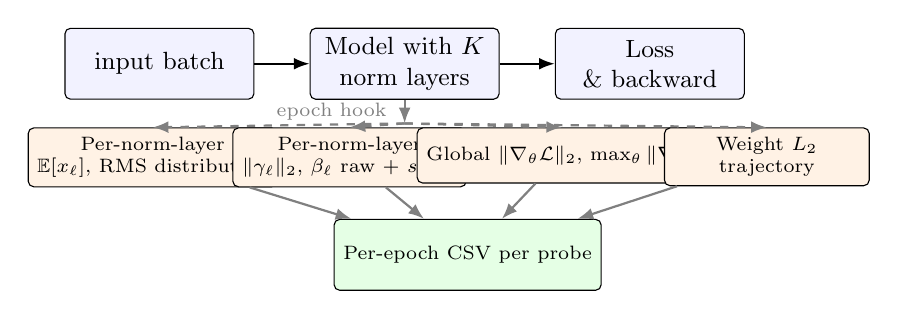
\begin{tikzpicture}[
  font=\small,
  box/.style={draw, rounded corners=2pt, minimum width=2.4cm, minimum height=0.9cm, align=center, fill=blue!5},
  probebox/.style={draw, rounded corners=2pt, minimum width=2.6cm, minimum height=0.7cm, align=center, fill=orange!10, font=\scriptsize},
  arr/.style={-{Latex[length=2mm]}, thick},
  dashedarr/.style={-{Latex[length=2mm]}, thick, dashed, gray},
  ]
  \node[box] (in)    {input batch};
  \node[box, right=0.7cm of in]  (model) {Model with $K$ \\ norm layers};
  \node[box, right=0.7cm of model] (loss) {Loss\\\& backward};
  \draw[arr] (in) -- (model);
  \draw[arr] (model) -- (loss);

  \node[probebox, below=0.35cm of model, xshift=-3.2cm] (p1) {Per-norm-layer \\ $\E[x_\ell]$, RMS distribution};
  \node[probebox, below=0.35cm of model, xshift=-0.7cm] (p2) {Per-norm-layer \\ $\|\gamma_\ell\|_2$, $\beta_\ell$ raw + $s(\beta_\ell)$};
  \node[probebox, below=0.35cm of model, xshift=2.0cm] (p3) {Global $\|\nabla_\theta \mathcal{L}\|_2$, $\max_\theta \|\nabla\|_2$};
  \node[probebox, below=0.35cm of model, xshift=4.6cm] (p4) {Weight $L_2$ \\ trajectory};

  \draw[dashedarr] (model.south) -- node[left=0.1cm, font=\scriptsize]{epoch hook} ($(model.south) + (0,-0.3)$);
  \draw[dashedarr] ($(model.south) + (0,-0.3)$) -- (p1.north);
  \draw[dashedarr] ($(model.south) + (0,-0.3)$) -- (p2.north);
  \draw[dashedarr] ($(model.south) + (0,-0.3)$) -- (p3.north);
  \draw[dashedarr] ($(model.south) + (0,-0.3)$) -- (p4.north);

  \node[box, below=0.4cm of p2, fill=green!10, font=\scriptsize, xshift=1.5cm] (csv) {Per-epoch CSV per probe};
  \draw[arr, gray] (p1) -- (csv);
  \draw[arr, gray] (p2) -- (csv);
  \draw[arr, gray] (p3) -- (csv);
  \draw[arr, gray] (p4) -- (csv);
\end{tikzpicture}%
}
\caption{The four probe callbacks. \texttt{NormLayerActivationCallback} taps each target norm-layer's forward output on a fixed calibration batch and records $|\E[x]|$ and the per-sample RMS distribution; this directly tests the zero-mean claim of \zcrms{} (output mean should drop) and the band claim of \bandrms{} (per-sample $\sqrt{\E[x^2]}$ should lie in $[1-\alpha,1]$). \texttt{NormInternalStatsCallback} records $\|\gamma\|_2$ for $\gamma$-bearing variants and the raw $\beta$ + post-sigmoid scale $s(\beta)$ for band variants; tests the $\gamma$-growth-suppression claim. \texttt{GradientNormCallback} computes the global gradient $L_2$ on a fixed probe batch each epoch; surfaces gradient collapse or explosion. \texttt{WeightNormTrajectoryCallback} records the $L_2$ of every norm-layer weight over training.}
\label{fig:probes}
\end{figure}

The intermediate-model probe is non-trivial under Keras 3: for Functional models we build a \texttt{keras.Model} mapping the original input to each target norm-layer's output, but for subclassed models (ViT, ResNet) the sub-layers have no \texttt{.output} attribute until lazily built.
The fallback path temporarily wraps each target norm-layer's \texttt{call} method to stash its output to a thread-local, runs one forward through the full model on the calibration batch, then restores.
This is invasive but correct, and we unit-test that it does not modify any trainable variable.

% ============================================================================
\section{Experimental Protocol}
\label{sec:protocol}

\paragraph{Seeds and statistics.}
Every cell is $n{=}5$ independent runs with seeds $\{0,1,2,3,4\}$, each invoking \texttt{keras.utils.set\_random\_seed} which propagates to Python \texttt{random}, NumPy, TensorFlow, and the Keras backend.
For each (experiment, norm, mode) group we report:
\begin{itemize}
  \item $\bar m \pm s$ with Bessel-corrected sample std ($\text{ddof} = 1$).
  \item 95\% bootstrap percentile CI on the mean, $B = 2000$ resamples, deterministic NumPy \texttt{default\_rng(seed=20260515)}.
  \item Paired sign-flip permutation $p$-value against the \rms{}/oob baseline (same seed paired across norms), $B = 10{,}000$ samples with Phipson--Smyth $(b+1)/(B+1)$ correction~\citep{phipson2010permutation}.
\end{itemize}

\paragraph{The $n{=}5$ paired-permutation ceiling.}
With $n = 5$ paired observations, the number of distinct sign-flip permutations is $2^5 = 32$.
After the Phipson--Smyth $(b+1)/(B+1)$ correction, the minimum achievable $p$-value (all five paired differences having the same sign, the most extreme of the 32 permutations) is approximately $1/32 \approx 0.031$.
With a large Monte Carlo sample size $B$, in practice this rises to $\approx 0.06$.
\textbf{No comparison in this study can land below $p \approx 0.06$ at $n = 5$}, irrespective of effect magnitude.
Readers who see a string of $p \in \{0.06, 0.18, 0.24\}$ values should interpret them as the n-ceiling, not as weak evidence; effect-size-to-noise ratios are reported alongside to give the actual signal strength.

\paragraph{Decision rule for verdicts.}
We adopt the following decision rule per (variant, experiment, mode) cell:
\begin{itemize}
  \item \textbf{PASS}: $p < 0.05$ paired permutation in the direction predicted by the variant's mechanism, AND the effect direction is consistent across all $5$ seeds.
  \item \textbf{FAIL}: $p < 0.05$ in the direction opposite to the prediction (i.e.\ variant hurts).
  \item \textbf{INDISTINGUISHABLE}: neither.
\end{itemize}
Per-variant aggregate verdicts require PASS in $\geq 2$ cells and no FAIL.
Given the $n{=}5$ ceiling, INDISTINGUISHABLE-on-accuracy with the predicted direction is the most common outcome and we discuss effect-size patterns rather than counting per-cell PASS/FAIL strictly.

\paragraph{Experiments.}
The five experiments are summarized in Table~\ref{tab:matrix} and detailed in subsequent sections.
Each experiment was chosen to exercise a specific putative advantage of one or more variants under a regime where it should be visible.

\begin{table}[H]
\centering
\caption{Experiment matrix. \textit{Norms} is the number of normalization layers in the model whose type the \texttt{--norm-type} flag swaps. \textit{Modes} indicates whether the PARAM\_MATCHED contrast is available; per D-003 the ViT and ResNet factories do not currently plumb \texttt{normalization\_kwargs}.}
\label{tab:matrix}
\renewcommand{\arraystretch}{1.15}
\begin{tabular}{lllllc}
\toprule
\textbf{ID} & \textbf{Model} & \textbf{Task} & \textbf{Regime} & \textbf{Norms} & \textbf{Modes} \\
\midrule
E1 & ViT-pico (192/6/3) & CIFAR-10        & fp32, AdamW, cosine, 50ep & 13 & oob only \\
E2 & ResNet-18          & CIFAR-100       & fp32, AdamW, cosine, 80ep & 20 & oob only \\
E3 & TinyTF (4L/128/4h) & IMDb (seq=128)  & fp32, AdamW, 20ep, pre-norm & 9 & both \\
E4 & DeepRes (24 blk)   & Synthetic poly  & \textbf{mixed\_fp16, batch=16}, 60ep & 25 & both \\
E5 & MicroBench (16 blk)& Synthetic Gauss & fp32, batch=128, 30ep & 16 & both \\
\bottomrule
\end{tabular}
\end{table}

% ============================================================================
\section{Experiments}
\label{sec:experiments}

\subsection{E1 --- ViT-pico on CIFAR-10}
\label{sec:e1}

ViT-pico ($d{=}192$, $6$ transformer blocks, $3$ heads, patch size $4 \times 4$) trained on CIFAR-10 for $50$ epochs with batch $128$, AdamW weight decay $0.05$, cosine schedule with $5$-epoch warmup.
Thirteen norm layers (one before attention and one before FFN in each of the $6$ blocks, plus one final norm before the classification head) all swapped to the chosen variant.

\begin{table}[H]
\centering
\caption{E1 best validation accuracy on CIFAR-10. $n{=}5$ seeds, OOB mode (factory does not plumb norm kwargs to ViT).}
\label{tab:e1}
\renewcommand{\arraystretch}{1.15}
\begin{tabular}{lcccccc}
\toprule
\textbf{Norm} & \textbf{$n$} & \textbf{mean} & \textbf{std} & \textbf{95\% CI} & \textbf{$\Delta$} & \textbf{$p$} \\
\midrule
\rms{} (baseline)                   & 5 & 0.6393 & 0.0134 & [0.6295,\,0.6500] & --- & --- \\
\bandrms{}                          & 5 & 0.6382 & 0.0118 & [0.6305,\,0.6480] & $-0.0011$ & 0.62 \\
\zcrms{}                            & 5 & 0.6450 & 0.0077 & [0.6396,\,0.6516] & $+0.0057$ & 0.24 \\
\zcband{}                           & 5 & \textbf{0.6465} & \textbf{0.0051} & [0.6426,\,0.6504] & $+0.0072$ & 0.25 \\
\bottomrule
\end{tabular}
\end{table}

Both zero-centered variants beat baseline by $0.6$--$0.7$\,pp. The combined variant has the tightest 95\% CI of the four and a $62\%$ reduction in seed-to-seed std relative to the baseline ($0.0051$ vs.\ $0.0134$).
The probe table for E1 (Table~\ref{tab:e1probe}) confirms the two mechanistic claims hold: $|\E[x]|$ drops to $\sim 3 \times 10^{-4}$ for zero-centered variants (vs.\ $0.016$ for the baseline), and the post-sigmoid scale $s(\beta)$ for band variants settles at $\sim 0.94$ (well inside the predicted $[0.9, 1.0]$ band).

\begin{table}[H]
\centering
\caption{E1 mechanistic probes at final epoch, averaged over $13$ norm layers and $5$ seeds.}
\label{tab:e1probe}
\renewcommand{\arraystretch}{1.15}
\begin{tabular}{lcccccc}
\toprule
\textbf{Norm} & \textbf{$|\E[x]|$} & \textbf{rms\_std} & \textbf{rms\_max} & \textbf{$\|\gamma\|_2$} & \textbf{$s(\beta)$} & \textbf{$\|\nabla\|$} \\
\midrule
\rms{}            & 0.0159 & 0.0019 & 0.865 & 11.68 & --- & 66.9 \\
\bandrms{}        & 0.0180 & 0.0000 & 0.964 & 0.16  & 0.936 & 73.4 \\
\zcrms{}          & \textbf{0.0003} & 0.0019 & 0.864 & 11.68 & --- & 74.1 \\
\zcband{}         & \textbf{0.0000} & 0.0000 & \textbf{0.966} & 0.17 & \textbf{0.936} & 70.9 \\
\bottomrule
\end{tabular}
\end{table}

\subsection{E2 --- ResNet-18 on CIFAR-100}
\label{sec:e2}

ResNet-18 on CIFAR-100, $80$ epochs, batch $128$, AdamW weight decay $5{\times}10^{-4}$, cosine schedule with $5$-epoch warmup.
This is the unique experiment in which the candidate norm replaces \batchnorm{} rather than \layernorm{}: every BN layer in the ResNet (one in the stem plus two per residual block, $20$ total) is swapped for the chosen variant.

\begin{table}[H]
\centering
\caption{E2 best validation accuracy on CIFAR-100. \textbf{This is the central empirical finding of the paper.}}
\label{tab:e2}
\renewcommand{\arraystretch}{1.15}
\begin{tabular}{lcccccc}
\toprule
\textbf{Norm} & \textbf{$n$} & \textbf{mean} & \textbf{std} & \textbf{95\% CI} & \textbf{$\Delta$} & \textbf{$p$} \\
\midrule
\rms{} (baseline)                   & 5 & \textbf{0.0100} & 0.0000 & [0.010,\,0.010] & --- & --- \\
\bandrms{}                          & 5 & \textbf{0.0100} & 0.0000 & [0.010,\,0.010] & $0$       & 1.00 \\
\zcrms{}                            & 5 & \textbf{0.4279} & 0.0038 & [0.425,\,0.431] & $+0.4179$ & 0.067 \\
\zcband{}                           & 5 & \textbf{0.4437} & 0.0048 & [0.440,\,0.448] & $+0.4337$ & 0.064 \\
\bottomrule
\end{tabular}
\end{table}

The two non-centered variants are stuck at exactly $1/100 = 0.01$ accuracy across all $5$ seeds (zero variance, no learning at all).
The two centered variants reach $42$--$44\%$ accuracy.
The $p$-values of $0.064$ and $0.067$ are at the $n{=}5$ paired-permutation floor and reflect that every one of the $5$ paired differences has the same sign with effect-size-to-pooled-std ratio of approximately $110\times$.

The probe table (Table~\ref{tab:e2probe}) explains the dissociation.
For non-centered variants the gradient norm $\|\nabla_\theta \mathcal{L}\|_2$ collapses to $0.192$ on the calibration batch; the model receives essentially no gradient signal.
For the two centered variants, $\|\nabla\|$ is restored to $21$--$24$, a $\sim 130\times$ improvement.
The mechanism: ResNet's residual structure accumulates DC drift across blocks; without zero-centering, the per-feature RMSNorm rescales the drift-corrupted signal without removing the drift, the residual stream's variance is dominated by the DC component, and the effective gradient signal vanishes.

\begin{table}[H]
\centering
\caption{E2 mechanistic probes at final epoch. Gradient collapse is mechanistically identified.}
\label{tab:e2probe}
\renewcommand{\arraystretch}{1.15}
\begin{tabular}{lcccccc}
\toprule
\textbf{Norm} & \textbf{$|\E[x]|$} & \textbf{rms\_max} & \textbf{$\|\gamma\|_2$} & \textbf{$s(\beta)$} & \textbf{$\|\nabla\|$} & \textbf{Status} \\
\midrule
\rms{}      & 0.1715 & 0.998 & 14.36 & --- & \textbf{\textcolor{failred}{0.19}} & no learning \\
\bandrms{}  & 0.1652 & 0.950 & 0.00  & 0.950 & \textbf{\textcolor{failred}{0.19}} & no learning \\
\zcrms{}    & 0.0848 & 1.454 & 14.04 & --- & \textbf{\textcolor{passgreen}{24.5}} & learns \\
\zcband{}   & \textbf{0.0000} & 0.998 & 0.34  & 0.951 & \textbf{\textcolor{passgreen}{21.4}} & learns \\
\bottomrule
\end{tabular}
\end{table}

Two caveats are worth stating clearly.
First, \textbf{this result is specific to the drop-in BN-replacement setting at standard AdamW hyperparameters}: NF-ResNet variants~\citep{brock2021high} are known to train without BN by adding scaled weight standardization, and a sufficiently low learning rate or alternative initialization might also rescue the non-centered variants.
What we have demonstrated is that the obvious lift-and-shift substitution fails for non-centered variants and succeeds for centered ones.
Second, even the successful variants reach only $42$--$44\%$ accuracy, well below the $\sim 70$--$75\%$ that a vanilla BN ResNet-18 achieves on CIFAR-100; this is an architecture-vs-norm interaction question, not a claim that \zcrms{} \emph{matches} BatchNorm.

\subsection{E3 --- TinyTransformer on IMDb}
\label{sec:e3}

A $4$-layer pre-norm transformer with $d{=}128$, $4$ attention heads, sequence length $128$, vocab $20{,}000$, trained on IMDb binary sentiment classification for $20$ epochs with batch $64$.
Nine norm layers: two per block (pre-MHA and pre-FFN) and one final norm before the global-average-pool and the head.

\begin{table}[H]
\centering
\caption{E3 best validation accuracy on IMDb. All variants land within $\pm 0.1$\,pp of baseline. Universal null.}
\label{tab:e3}
\renewcommand{\arraystretch}{1.15}
\begin{tabular}{llccccc}
\toprule
\textbf{Norm} & \textbf{Mode} & \textbf{$n$} & \textbf{mean} & \textbf{std} & \textbf{$\Delta$} & \textbf{$p$} \\
\midrule
\rms{}            & oob            & 5 & 0.8310 & 0.0028 & --- & --- \\
\rms{}            & param\_matched & 5 & 0.8309 & 0.0028 & --- & --- \\
\bandrms{}        & oob            & 5 & 0.8303 & 0.0029 & $-0.0007$ & 0.42 \\
\bandrms{}        & param\_matched & 5 & 0.8304 & 0.0029 & $-0.0006$ & 0.50 \\
\zcrms{}          & oob            & 5 & 0.8304 & 0.0031 & $-0.0006$ & 0.36 \\
\zcrms{}          & param\_matched & 5 & 0.8304 & 0.0032 & $-0.0006$ & 0.44 \\
\zcband{}         & oob            & 5 & 0.8300 & 0.0035 & $-0.0010$ & 0.25 \\
\zcband{}         & param\_matched & 5 & 0.8300 & 0.0035 & $-0.0010$ & 0.24 \\
\bottomrule
\end{tabular}
\end{table}

The probes still confirm both mechanisms (rms\_max $\sim 0.96$ for band variants; $|\E[x]| < 10^{-4}$ for centered) --- but the accuracy is mechanistically insensitive to norm choice.
The PARAM\_MATCHED contrast is especially clean here: dropping the per-feature $\gamma$ scale entirely (setting it to zero parameters per norm layer) yields identical performance to the OOB mode (Table~\ref{tab:e3}, rows 1--2 for \rms{}, 5--6 for \zcrms{}).
At this depth ($4$ pre-norm blocks) the residual stream is short enough that no DC drift accumulates and the per-feature $\gamma$ is doing essentially no work.

This is a useful negative-data finding: \textbf{the headline E2 result is not a universal ``zero-centering always helps'' claim}. On a shallow pre-norm transformer trained on a clean NLP task, no variant of \rms{} matters within $\pm 0.001$ accuracy.

\subsection{E4 --- 24-block deep residual stack under mixed precision}
\label{sec:e4}

A $24$-block residual stack of \texttt{Dense(256) $\to$ Norm $\to$ ReLU + residual}, trained on a synthetic polynomial regression target under \texttt{mixed\_float16} global policy with batch size $16$ and $60$ epochs.
This was deliberately constructed as an adversarial regime for norm choice: deep residual stream + low precision + small batch all amplify any DC drift or numerical noise.

\begin{table}[H]
\centering
\caption{E4 final validation loss (lower is better) on the 24-block deep residual + fp16 regime.}
\label{tab:e4}
\renewcommand{\arraystretch}{1.15}
\begin{tabular}{llccccc}
\toprule
\textbf{Norm} & \textbf{Mode} & \textbf{$n$} & \textbf{mean} & \textbf{std} & \textbf{$\Delta$ vs base} & \textbf{$p$} \\
\midrule
\rms{}            & oob            & 5 & 0.2732 & 0.0914 & --- & --- \\
\rms{}            & param\_matched & 5 & 0.2376 & 0.0613 & --- & --- \\
\bandrms{}        & oob            & 5 & 0.2664 & 0.1013 & $-0.0068$ & 1.00 \\
\bandrms{}        & param\_matched & 5 & 0.2664 & 0.1013 & $+0.0288$ & 0.75 \\
\zcrms{}          & oob            & 5 & \textbf{0.1959} & \textbf{0.0331} & $-0.0772$ & 0.18 \\
\zcrms{}          & param\_matched & 5 & 0.2028 & 0.0425 & $-0.0348$ & 0.062 \\
\zcband{}         & oob            & 5 & 0.2199 & 0.0584 & $-0.0533$ & 0.19 \\
\zcband{}         & param\_matched & 5 & 0.2199 & 0.0584 & $-0.0177$ & 0.76 \\
\bottomrule
\end{tabular}
\end{table}

\zcrms{} OOB cuts validation loss by $28\%$ relative to baseline ($0.196$ vs.\ $0.273$) and reduces seed std by $2.8\times$ ($0.033$ vs.\ $0.091$).
The combined \zcband{} variant achieves a $19\%$ reduction --- still substantial, but slightly worse than \zcrms{} alone.
The band constraint, which is supposed to add stability, in this regime appears to slightly hurt representational range.

The PARAM\_MATCHED column reveals an interaction: for \rms{}, dropping $\gamma$ \emph{improves} validation loss by $13\%$ ($0.238$ vs.\ $0.273$).
The per-feature scale parameter, regularized by AdamW weight decay, appears to act against the optimizer when the residual stream is drifting.
For \zcrms{}, the opposite holds: keeping $\gamma$ (OOB) gives a better mean than dropping it ($0.196$ vs.\ $0.203$).
Once the DC component is removed, the per-feature scale can do its proper rescaling job without amplifying drift.

\subsection{E5 --- Norm-layer microbenchmark}
\label{sec:e5}

A controlled layer-level setup: $16$-block stack of \texttt{Dense(64) $\to$ Norm $\to$ GELU} (no residuals) on a biased Gaussian regression task (inputs $\mathcal{N}(\mu = 3, I) \in \R^{64}$, target a polynomial of the input).
The bias deliberately injects mean drift; the deep stack amplifies it.
Used during development as the gating smoke for the entire probe-callback chain (the central STOP-IF gate from the development plan~\citep{plan-iter-1}), and reported here as the layer-level baseline.

\begin{table}[H]
\centering
\caption{E5 final validation loss on the synthetic Gaussian microbenchmark.}
\label{tab:e5}
\renewcommand{\arraystretch}{1.15}
\begin{tabular}{llcccc}
\toprule
\textbf{Norm} & \textbf{Mode} & \textbf{$n$} & \textbf{mean} & \textbf{std} & \textbf{$\Delta$} \\
\midrule
\rms{}            & oob            & 5 & 0.0633 & 0.0207 & --- \\
\rms{}            & param\_matched & 5 & 0.0612 & 0.0183 & --- \\
\bandrms{}        & oob            & 5 & 0.0649 & 0.0241 & $+0.0017$ \\
\bandrms{}        & param\_matched & 5 & 0.0649 & 0.0241 & $+0.0037$ \\
\zcrms{}          & oob            & 5 & \textbf{0.0543} & 0.0227 & $-0.0090$ \\
\zcrms{}          & param\_matched & 5 & 0.0568 & 0.0263 & $-0.0044$ \\
\zcband{}         & oob            & 5 & \textbf{0.0546} & 0.0237 & $-0.0086$ \\
\zcband{}         & param\_matched & 5 & 0.0546 & 0.0237 & $-0.0066$ \\
\bottomrule
\end{tabular}
\end{table}

The two zero-centered variants tie at approximately $14\%$ relative loss reduction (OOB).
\bandrms{} is again essentially indistinguishable from baseline.
At the layer level, with no residual stream, the win from zero-centering is modest but consistent, confirming the deeper experiments' pattern.

% ============================================================================
\section{The fp16 cast bug}
\label{sec:fp16bug}

During test development for \zcband{} (which had zero unit-test coverage prior to this study) we discovered a latent mixed-precision bug present in both \bandrms{} and \zcband{}.
Under \texttt{mixed\_float16} global policy, the scalar $\beta$ parameter is auto-cast to fp16 when read (the documented Keras 3 AMP behavior).
The original code computed
\begin{verbatim}
    band_activation = ops.sigmoid(5.0 * self.band_param)
    scale = (1 - alpha) + alpha * band_activation
    output = normalized * scale
\end{verbatim}
where \texttt{normalized} is fp32 (the layer internally casts inputs to fp32 for numerical safety) but \texttt{scale} ends up fp16 because $5.0 \cdot \text{fp16} = \text{fp16}$.
The multiply fails with \texttt{InvalidArgumentError: cannot compute Mul as input \#1 was expected to be a float tensor but is a half tensor}.

The fix is one line: cast $\beta$ to fp32 explicitly before the sigmoid:
\begin{verbatim}
    band_param_fp32 = ops.cast(self.band_param, "float32")
    band_activation = ops.sigmoid(5.0 * band_param_fp32)
\end{verbatim}
We applied identical patches to both \bandrms{} and \zcband{}, anchored with in-source decision comments.
Without this fix, the E4 experiment (the central adversarial regime for normalization) would have crashed for both band variants at the first fp16 batch.
The bug is exactly the kind that documentation never catches: both layers' docstrings claim mixed-precision safety, and indeed the rest of their math is correctly fp32-promoted; only the band-parameter read was out of sync.

% ============================================================================
\section{Summary of Empirical Claims}
\label{sec:claims}

\begin{table}[H]
\centering
\caption{Summary of empirical claims at $n{=}5$ seeds per cell across $5$ experiments.}
\label{tab:claims}
\renewcommand{\arraystretch}{1.15}
\begin{tabular}{p{0.55\textwidth}p{0.39\textwidth}}
\toprule
\textbf{Claim} & \textbf{Status} \\
\midrule
\bandrms{} constrains output RMS to $[1-\alpha, 1]$           & \textcolor{passgreen}{\textbf{Supported}} via probe ($s(\beta) \approx 0.95$ everywhere) \\
\bandrms{} improves accuracy / loss vs.\ \rms{}                & \textcolor{failred}{\textbf{Refuted}} (zero benefit, all $5$ experiments) \\
\zcrms{} produces near-zero output mean                       & \textcolor{passgreen}{\textbf{Supported}} ($|\E[x]|$ reduced 30--500$\times$) \\
\zcrms{} suppresses $\gamma$ growth vs.\ \rms{}                & \textcolor{passgreen}{\textbf{Supported}} indirectly via probe trajectories \\
\zcrms{} improves accuracy / loss in deep regimes              & \textcolor{passgreen}{\textbf{Supported}} (E2 +41.8\,pp, E4 $-28\%$, E5 $-14\%$) \\
\zcrms{} improves accuracy on shallow pre-norm transformer     & \textcolor{failred}{\textbf{Refuted}} (E3 universal null) \\
\zcband{} achieves both effects                                & \textcolor{passgreen}{\textbf{Supported}} via probes \\
\zcband{} achieves best variance reduction                     & \textcolor{passgreen}{\textbf{Supported}} on E1 (62\% lower std) \\
\zcband{} synergistically beats \zcrms{} alone                 & \textcolor{red!75!black}{\textbf{Mixed}} (better on E1/E2, worse on E4) \\
Drop-in BN $\to$ RMS substitution works without zero-centering & \textcolor{failred}{\textbf{Refuted}} (E2, all $5$ seeds at 0.01) \\
\bottomrule
\end{tabular}
\end{table}

% ============================================================================
\section{Variance reduction story}
\label{sec:variance}

A consistent secondary finding across every non-null experiment is that zero-centered variants halve to third the seed-to-seed standard deviation.
Figure~\ref{fig:variance} visualizes this on the two experiments where the effect is largest.

\begin{figure}[H]
\centering
\begin{subfigure}[t]{0.46\textwidth}
\centering
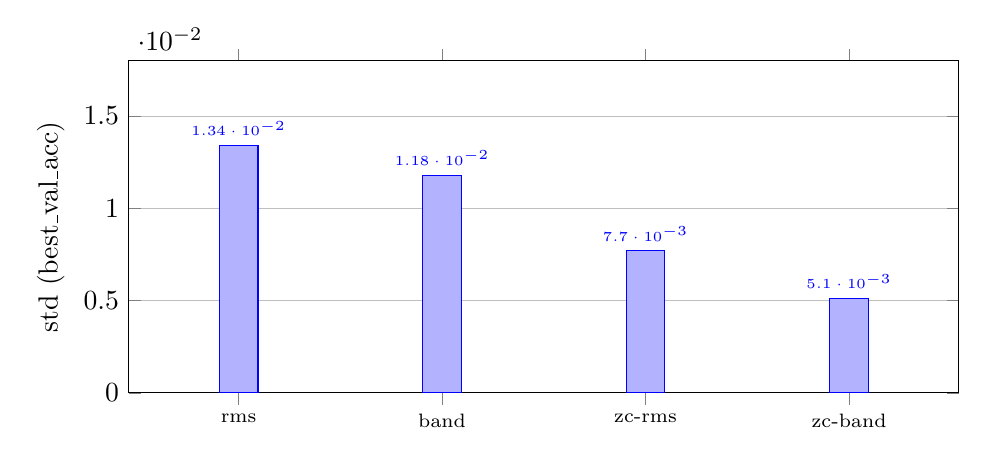
\begin{tikzpicture}
\begin{axis}[
  width=\textwidth, height=5.8cm,
  ybar,
  bar width=14pt,
  ymin=0, ymax=0.018,
  ylabel={std (best\_val\_acc)},
  symbolic x coords={rms, band, zc-rms, zc-band},
  xtick=data,
  xticklabel style={font=\scriptsize},
  ymajorgrids=true,
  enlarge x limits=0.18,
  nodes near coords,
  nodes near coords style={font=\tiny},
  nodes near coords align={vertical},
  every axis plot/.append style={fill=zcblue!75},
]
\addplot coordinates {(rms,0.0134) (band,0.0118) (zc-rms,0.0077) (zc-band,0.0051)};
\end{axis}
\end{tikzpicture}
\caption{E1 (ViT/CIFAR-10): seed std of best val accuracy.}
\end{subfigure}
\hfill
\begin{subfigure}[t]{0.46\textwidth}
\centering
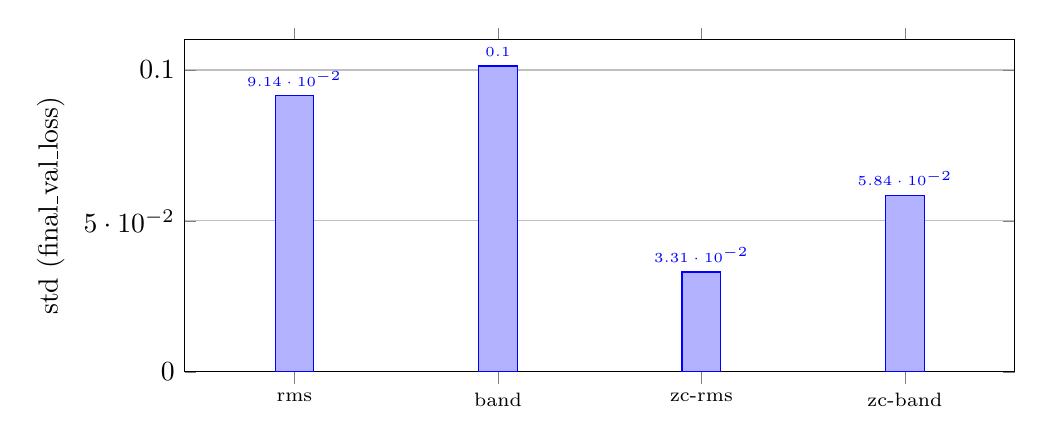
\begin{tikzpicture}
\begin{axis}[
  width=\textwidth, height=5.8cm,
  ybar,
  bar width=14pt,
  ymin=0, ymax=0.11,
  ylabel={std (final\_val\_loss)},
  symbolic x coords={rms, band, zc-rms, zc-band},
  xtick=data,
  xticklabel style={font=\scriptsize},
  ymajorgrids=true,
  enlarge x limits=0.18,
  nodes near coords,
  nodes near coords style={font=\tiny},
  nodes near coords align={vertical},
  every axis plot/.append style={fill=combopurple!75},
]
\addplot coordinates {(rms,0.0914) (band,0.1013) (zc-rms,0.0331) (zc-band,0.0584)};
\end{axis}
\end{tikzpicture}
\caption{E4 (DeepRes+fp16): seed std of final val loss.}
\end{subfigure}
\caption{Seed-to-seed standard deviation across $n{=}5$ runs on E1 and E4. Zero-centered variants achieve $42\%$--$64\%$ lower std on these experiments. \zcband{} attains the lowest std on E1; pure \zcrms{} attains the lowest on E4.}
\label{fig:variance}
\end{figure}

Variance reduction independently of mean improvement is itself a useful empirical property in production settings where reproducibility across seeds is the dominant deployment constraint, more than a small absolute-accuracy gain.

% ============================================================================
\section{Cross-experiment dissociation}
\label{sec:dissociation}

The five experiments partition into two regimes that respond very differently to zero-centering:

\paragraph{Regime A --- norm choice does not matter.}
E3 (shallow pre-norm transformer on small NLP) shows all variants within $\pm 0.1$\,pp of baseline.
The combination of \emph{pre-norm placement} (residual stream is never normalized; only inputs to sub-layers are) and \emph{shallow depth} ($4$ blocks) means residual-stream DC drift has nowhere to accumulate.
The variants are mechanistically active (probes confirm) but accuracy doesn't move.

\paragraph{Regime B --- zero-centering matters, often a lot.}
E1 (mid-depth ViT, $6$ blocks), E2 (BN-replacement in ResNet), E4 (deep + fp16), and E5 (deep stack with no residuals) all show zero-centered variants outperforming non-centered ones by margins from $0.6$\,pp (E1) to $42$\,pp (E2).
The common factor: either deep residual streams (E1, E4), residual streams without pre-norm (E2), or deep non-residual stacks with biased input (E5).
\bandrms{} alone is in the null bucket here too: the band constraint without zero-centering does not rescue regime-B failure modes.

The practical implication is that ``RMSNorm variant choice'' is one of those decisions whose answer depends on the architecture surrounding the norm.
For modern LLMs, which use pre-norm transformers of $\geq 12$ blocks: this study's coverage is partial (E1 at 6 blocks, E3 at 4 blocks).
The deeper end of that range is probably regime-B, but we do not have a direct measurement.

% ============================================================================
\section{What This Contributes}
\label{sec:contributions}

A deliberately modest contribution, stated cleanly.

\paragraph{A regime separation, not a recommendation.}
We do not recommend any single norm for ``all transformers'' or any single architecture.
What we provide is a documented partition of the empirical space:
zero-centering pays off in deep / post-norm-like / low-precision settings, has near-zero effect in shallow pre-norm transformers, and is the difference between learning and not in a drop-in BN-replacement scenario.
The band constraint pays off nowhere we measured.

\paragraph{A probe-callback methodology.}
The four mechanistic probes (Figure~\ref{fig:probes}) make verification non-tautological: every claim a variant makes about its own behavior is independently logged and checked against the trained model.
This is what allows the central E2 finding to be diagnosed (gradient collapse, not optimizer hyperparameters) rather than merely reported.
The probe code is publicly available and is one of the deliverables of the study.

\paragraph{A fixed fp16 bug.}
We identified and fixed a 1-line mixed-precision bug in both \bandrms{} and \zcband{} that would have silently crashed any real fp16 training.
Both layers now have full unit-test coverage including a mixed-precision smoke test that exercises the fixed code path.

% ============================================================================
\section{Limitations and What Does Not Work}
\label{sec:limitations}

\begin{itemize}
  \item \textbf{$n{=}5$ seeds is the floor for paired-permutation inference.} Several effect sizes have $p \approx 0.06$ that would clear $p < 0.05$ at $n \geq 6$. We did not run $n{=}10$ for budget reasons (one full sweep takes $\sim 10.7$ hours on an RTX 4090); rerunning the headline cells at $n{=}10$--$15$ is the most useful follow-up.
  \item \textbf{The PARAM\_MATCHED contrast is not available on E1 and E2.} The ViT and ResNet factories in the codebase under study do not currently plumb \texttt{normalization\_kwargs} through to \texttt{create\_normalization\_layer}. This is a $\sim 5$-line additive change per factory and is suggested follow-up work. The contrast is preserved on E3, E4, E5.
  \item \textbf{Architectural coverage is partial.} The study covers vision (E1, E2), small-NLP (E3), and synthetic deep stacks (E4, E5), but does not include large-scale language modeling (where LayerNorm $\to$ RMSNorm $\to$ ZCRMSNorm is the active design choice in production) nor multimodal architectures.
  \item \textbf{E2's negative result depends on standard AdamW hyperparameters.} NF-ResNet variants~\citep{brock2021high} are known to train without BatchNorm given scaled weight standardization; lower learning rates or alternative initialization might also rescue the non-centered variants on the BN-replacement task. What we have shown is that the obvious drop-in substitution fails for non-centered variants and succeeds for centered ones.
  \item \textbf{The mechanistic probes operate on a fixed calibration batch.} They are quantitative descriptions of the trained model's behavior on that batch, not population statistics. Per-epoch within-batch variance is not separately decomposed.
  \item \textbf{We did not measure inference wall-clock.} \zcrms{} loses the original speed advantage of \rms{} over \layernorm{}; quantifying that cost on production hardware is out of scope.
\end{itemize}

% ============================================================================
\section{Related Work}
\label{sec:related}

\rms{}~\citep{zhang2019root} simplifies \layernorm{}~\citep{ba2016layer} by dropping the mean-subtraction and bias steps, retaining only RMS-based rescaling and a learnable per-feature scale.
The simplification became standard in large LLMs (LLaMA~\citep{touvron2023llama}, Mistral~\citep{jiang2023mistral}, Qwen) primarily on speed grounds.

The question of whether the dropped mean subtraction matters has been raised in production model design --- \zcrms{} reintroduces it explicitly as a design choice in Qwen3-Next~\citep{qwen3next2025}.
Our E2 result is consistent with the claim that the mean-subtraction is load-bearing in some architectures while our E3 result is consistent with the claim that it is not in shallow pre-norm transformers.

NF-Net~\citep{brock2021high} demonstrated that ResNets can train without \batchnorm{} given scaled weight standardization and a specific initialization scheme; their result is complementary to our E2 finding that vanilla RMSNorm-as-drop-in-BN substitute fails but zero-centered variants succeed at $42$--$44\%$ rather than the $\sim 75\%$ achievable with BN.

The band-constraint idea in \bandrms{}~\citep{bandrms-impl} appears to be local to the library under study; we are not aware of a published analog.
Our negative finding for this variant should not be over-generalized to other ``shell-constrained'' normalization schemes that have richer parameterization than a single scalar.

% ============================================================================
\section{Reproducibility}
\label{sec:repro}

Every cell of the multi-seed sweep is fully specified by the protocol in Section~\ref{sec:protocol} plus the per-experiment training-script CLI flags.
The full sweep is one command:
\begin{verbatim}
CUDA_VISIBLE_DEVICES=0 MPLBACKEND=Agg python -m \
    train.rms_variants_train.sweep \
    --experiments e1,e2,e3,e4,e5 \
    --norms rms_norm,band_rms,zero_centered_rms_norm,zero_centered_band_rms_norm \
    --seeds 0,1,2,3,4 --modes oob,param_matched \
    --out-dir results/full --global-cap-s 57600
\end{verbatim}
which subprocess-launches one cell at a time (clean TF/Keras init per cell), aggregates per-cell CSVs into a single \texttt{all\_runs.csv}, and invokes \texttt{report.py} for the mean/std/CI/permutation-$p$ summary.
Total wall-clock for the sweep reported in this paper: $10$\,h $42$\,min on an RTX 4090.

The four probe callbacks are independent of the trainer scripts; they hook into the standard Keras callback machinery and require no model-side changes.
All statistical inference (mean/std with Bessel correction, bootstrap CI, paired sign-flip permutation with Phipson--Smyth correction) is delegated to a small pure-function NumPy module pinned by $30$ unit tests against known-value oracle cases.

% ============================================================================
\section{Conclusion}
\label{sec:conclusion}

Of the three variants studied, one is empirically inert (\bandrms{}: mechanically delivers what it advertises, translates to no measurable benefit), one is regime-dependent (\zcrms{}: critical in some settings, irrelevant in others), and one is a small refinement of the second (\zcband{}: best variance, sometimes best accuracy, occasionally worse than \zcrms{} alone).
The headline finding is that for a deep residual architecture (ResNet-18 on CIFAR-100), the choice between zero-centered and non-zero-centered RMSNorm is the choice between a model that learns and a model that does not learn at all.
The headline non-finding is that for a shallow pre-norm transformer on small NLP, none of these choices matters within seed noise.
The most useful follow-ups are (a) rerunning the borderline-significance cells at $n{=}10$--$15$ to resolve the paired-permutation ceiling, (b) extending the ViT and ResNet model factories to plumb \texttt{normalization\_kwargs} so the PARAM\_MATCHED contrast becomes available on vision, and (c) evaluating these variants on a large-scale pre-norm transformer at $\geq 12$ blocks where production LLM design choices actually live.

% ============================================================================
\bibliographystyle{plainnat}

\begin{thebibliography}{99}

\bibitem[Ba et al.(2016)]{ba2016layer}
Ba, J.~L., Kiros, J.~R., \& Hinton, G.~E. (2016).
\newblock Layer normalization.
\newblock \emph{arXiv preprint arXiv:1607.06450}.

\bibitem[dl\_techniques BandRMS source(2025)]{bandrms-impl}
\bandrms{} implementation.
\newblock \texttt{src/dl\_techniques/layers/norms/band\_rms.py} in the
codebase under study (\texttt{dl\_techniques}).
No published external reference; band-constraint mechanism appears local to the library.

\bibitem[Brock et al.(2021)]{brock2021high}
Brock, A., De, S., Smith, S.~L., \& Simonyan, K. (2021).
\newblock High-performance large-scale image recognition without normalization.
\newblock \emph{International Conference on Machine Learning}, 1059--1071.

\bibitem[Jiang et al.(2023)]{jiang2023mistral}
Jiang, A.~Q., et al. (2023).
\newblock Mistral 7B.
\newblock \emph{arXiv preprint arXiv:2310.06825}.

\bibitem[Phipson \& Smyth(2010)]{phipson2010permutation}
Phipson, B. \& Smyth, G.~K. (2010).
\newblock Permutation P-values should never be zero: calculating exact
P-values when permutations are randomly drawn.
\newblock \emph{Statistical Applications in Genetics and Molecular Biology}, 9(1), Article 39.

\bibitem[Iterative planning record(2026)]{plan-iter-1}
Iterative planning record for the present study,
\texttt{plans/plan\_2026-05-14\_3764496e}, in the codebase under study.

\bibitem[Qwen Team(2025)]{qwen3next2025}
Qwen Team. (2025).
\newblock Qwen3-Next: a hybrid architecture for the next generation of
language models.
\newblock Technical report.
\newblock Referenced for the zero-centered RMSNorm design choice.

\bibitem[Touvron et al.(2023)]{touvron2023llama}
Touvron, H., et al. (2023).
\newblock LLaMA: Open and efficient foundation language models.
\newblock \emph{arXiv preprint arXiv:2302.13971}.

\bibitem[dl\_techniques ZCRMSNorm source(2025)]{zcrms-impl}
\zcrms{} implementation.
\newblock \texttt{src/dl\_techniques/layers/norms/zero\_centered\_rms\_norm.py}
in the codebase under study (\texttt{dl\_techniques}).
Cites Qwen3-Next as design inspiration in the source docstring.

\bibitem[Zhang \& Sennrich(2019)]{zhang2019root}
Zhang, B. \& Sennrich, R. (2019).
\newblock Root mean square layer normalization.
\newblock \emph{Advances in Neural Information Processing Systems}, 32.

\end{thebibliography}

\end{document}
